
In this section, we introduce the technical details behind comparative reasoning.
We first introduce on what condition we need to exert pairwise reasoning for two pieces of clues (e.g., two edges/triples),
and then introduce two methods which focus on pairwise reasoning.
Finally, we present the collective comparative reasoning.
The main idea behind these functions is that we use a knowledge segment to express the semantic meaning of each query triple, and
check the inconsistency according to information in the knowledge segments.


\subsection{Pairwise Comparative Reasoning Condition}

%Given a pair of triples, we may don't need to check them if they talk about different things.
Given a pair of clues $<{\tt s_1}, {\tt p_1}, {\tt o_1}>$ and $<{\tt s_2}, {\tt p_2}, {\tt o_2}>$, we can divide it into the following six cases, including
\noindent
\begin{enumerate}[wide, labelwidth=!, labelindent=0pt]
\item [C1.]
{
${\tt s_1} \neq {\tt s_2}$, ${\tt s_1} \neq {\tt o_2}$, ${\tt o_1} \neq {\tt s_2}$, ${\tt o_1} \neq {\tt o_2}$.
For this case, these two clues apparently refer to different things,
e.g., $<${\tt Alan Turing}, {\tt wasBornIn}, {\tt United Kingdom}$>$ and $<${\tt Google}, {\tt isLocatedIn}, {\tt USA}$>$.
}
\item [C2.]
{
%Given $<{\tt s_1}, {\tt p_1}, {\tt o_1}>$ and $<{\tt s_2}, {\tt p_2}, {\tt o_2}>$, where
${\tt s_1} = {\tt s_2}$ and ${\tt o_1} = {\tt o_2}$.
If ${\tt p_1} = {\tt p_2}$, these two clues are the same.
If ${\tt p_1}$ and ${\tt p_2}$ are different or irrelevant, e.g., ${\tt p_1} ={\tt wasBornIn}$, ${\tt p_2} = {\tt hasWebsite}$,
these two clues refer to different things.
However, if ${\tt p_1}$ contradicts ${\tt p_2}$, they are inconsistent with each other.
}
\item [C3.]
{
%Given $<{\tt s_1}, {\tt p_1}, {\tt o_1}>$ and $<{\tt s_2}, {\tt p_2}, {\tt o_2}>$, where
${\tt s_1} = {\tt s_2}$ but ${\tt p_1} \neq {\tt p_2}$ and ${\tt o_1} \neq {\tt o_2}$, e.g., $<${\tt Alan Turing}, {\tt wasBornIn}, {\tt Maida Vale}$>$, $<${\tt Alan Turing}, {\tt livesIn}, {\tt United Kingdom}$>$.
}
\item [C4.]
{
%Given $<{\tt s_1}, {\tt p_1}, {\tt o_1}>$ and $<{\tt s_2}, {\tt p_2}, {\tt o_2}>$, where
${\tt s_1} = {\tt s_2}$, ${\tt p_1} = {\tt p_2}$, but ${\tt o_1} \neq {\tt o_2}$,
e.g., $<${\tt Alan Turing}, {\tt wasBornIn}, {\tt Maida Vale}$>$, $<${\tt Alan Turing}, {\tt wasBornIn}, {\tt United Kingdom}$>$.
}
\item [C5.]
{
%Given $<{\tt s_1}, {\tt p_1}, {\tt o_1}>$ and $<{\tt s_2}, {\tt p_2}, {\tt o_2}>$, where
${\tt o_1} = {\tt o_2}$, but ${\tt s_1} \neq {\tt s_2}$.
For this case, no matter what ${\tt p_1}$ and ${\tt p_2}$ are, these two clues refer to different things.
}
\item [C6.]
{
%Given $<{\tt s_1}, {\tt p_1}, {\tt o_1}>$ and $<{\tt s_2}, {\tt p_2}, {\tt o_2}>$, where
${\tt o_1} = {\tt s_2}$.
For this case, no matter what ${\tt p_1}$ and ${\tt p_2}$ are, they refer to different things.
For example, $<${\tt Alan Turing}, {\tt wasBornIn}, {\tt United Kingdom}$>$, $<${\tt United Kingdom}, {\tt dealsWith}, {\tt USA}$>$.
}
\end{enumerate}


%\vspace{-1\baselineskip}
Among these six cases, we can see that the clue pair in C1, C5 and C6 refer to different things. Therefore, there is no need to check the inconsistency between them. For C2, we only need to check the semantic meaning of their predicates, i.e., whether ${\tt p_1}$ contradicts ${\tt p_2}$. For example, ${\tt p_1} = {\tt isFather}$ and ${\tt p_2} = {\tt isSon}$, they are inconsistent with each other. Otherwise, there is no inconsistency between them.
%\hh{add details: e.g. if p1 is the opposite of p2, they are inconsistent. otherwise, there is no inconsistency.}.
We mainly focus on C3 and C4 where the two clues may be inconsistent with each other even if each of them is true. For example,
%in Figure ~\ref{inconsistency},
either $<${\tt Barack Obama}, {\tt graduatedFrom}, {\tt Harvard University}$>$ or $<${\tt Barack Obama}, {\tt majorIn} , {\tt Political Science}$>$
could be true. But putting them together, they cannot be both true, since
{\tt Barack Obama} majored in {\tt law} instead of {\tt Political Science} when he studied at {\tt Harvard University}.
%these two claims could not happen at the same time.
In other words, they are mutually exclusive with each other and thus are inconsistent.
However,
queries like $<${\tt Alan Turing}, {\tt wasBornIn}, {\tt Maida Vale}$>$ and $<${\tt Alan Turing}, {\tt wasBornIn}, {\tt United Kingdom}$>$ are both true, because {\tt Maida Vale} belongs to {\tt United Kingdom}. Alternatively, we can say that {\tt United Kingdom} contains {\tt Maida Vale}.
We summarize that if (1) the subjects of two clues are the same, and (2) their predicates are similar with each other or the same, they refer to the same thing. Furthermore, if their objects are two uncorrelated entities, it is highly likely that these two clues are inconsistent with each other.

Based on the above observations, we take the following three steps for pairwise comparative reasoning. First, given a pair of clues, we decide which of six cases it belongs to, by checking the subjects, predicates and objects of these two clues. Second, if this pair of clues belongs to C3 or C4, we need to further decide whether they are consistent with each other. In the following sections, we illustrate how to tackle this case.

\subsection{Neural Network Based Pairwise Comparative Reasoning}

Given two knowledge segments of a pair of clues which belong to C3 or C4,
we treat each knowledge segment as an attributed graph, and adopt some ideas from network alignment to facilitate comparative reasoning.
The basic idea is that if the two knowledge segments are consistent, most of their nodes must be able to align with or close to each other in the embedding space. Otherwise, the embedding distance of the inconsistent nodes should be large.
Generally, the inconsistent checking problem is similar to anomaly detection or dissimilarity detection problem in the embedding space.

When reasoning a pair of knowledge segments, we consider two kinds of information: structure information and semantic information. We envision that both of them are important. For example, in Figure ~\ref{inconsistency}, {\tt Air Force One} and {\tt Helicopter} have similar structure information because they have many common neighbors, but their semantic meanings are very different, this may indicate a potential inconsistency between the two knowledge segments. On the other hand, although {\tt Air Force One} and {\tt Helicopter} have different structure information (when considering edge type), they also have different semantic information. This prompts that they refer to the different things. Inspired by this observation, we propose a neural network model which considers both the structure information and semantic information of knowledge segments to achieve pairwise comparative reasoning.



To encode the structure similarity, we use random walk with restart (considering edge type) to encode the knowledge segment structure information. The similar idea has been used by many other works, e.g. ~\cite{Tong2006rdwalk}, ~\cite{bright}.
Given a set of anchor nodes, random walk with restart will calculate a score for each node in the knowledge segment w.r.t. each anchor node. If two nodes have the similar random walk with restart score vector, their structure similarity should be high.
To encode the semantic information of the knowledge segment, we borrow some ideas from natural language processing. More specifically, we sample some paths from the knowledge graph, and treat each path as a sentence, nodes in the knowledge graph can be treated as words in the sentence. If two nodes occur in the same sentence, their semantic information should be similar.


\subsubsection{Structure Embedding}

Given two knowledge segments, the common nodes in these two knowledge segments can be treated as anchor entities, structure embedding
aims to embed the nodes in the knowledge segments to a high dimension space while keeping their structure information.
The key intuition is that, the set of anchor links $\mathcal{L}$ provides the landmarks for all nodes in both networks. Relative positions based on anchor links can form a unified space for all nodes regardless which network they belong to ~\cite{bright}. Therefore, we can use random walk with restart to measure the relative position between nodes and anchor links.
Let $KS_1$ and $KS_2$ be the two knowledge segments.
Given an anchor link $l \in \mathcal{L}$ (we use $l_1$ and $l_2$ to denote the linked entities in $KS_1$ and $KS_2$),
the $\textrm{RWR}$ score vector $r_{l_1}$ of size $n_1 \times 1$ can be obtained
\begin{equation}
r_{l_1} = (1 - \beta)\hat{W_1} r_{l_1} + \beta e_{l_1}
\end{equation}
where $n_1$ is the number of nodes in $KS_1$, $\hat{W_1}$ is the row normalized adjacency matrix of $KS_1$, $\beta$ is the restart probability and $e_{l_1}$ is one-hot vector with  $e_{l_1}(l_1) = 1$ and all other entries are 0.
We can solve the equation and get the final expression of $r_{l_1}$ as:
\begin{equation}
r_{l_1} = \beta (I - (1 - \beta))\hat{W_1}^{-1} e_{l_1}
\end{equation}
Note that if $KS_1$ and $KS_2$ are the same, they will have the same random walk with restart score matrices.

After we get the  random walk with restart matrices, we then use a share neural network to learn the embedding of these two knowledge segments. In this way, the structure information of each node can be kept in the embedding space. The learned embedding for $KS_1$ can be calculated as:
\begin{equation}
E_{1} = \textrm{NeuralNetwork}(\textrm{RWR}_{1})
\end{equation}
where $\textrm{RWR}_{1}$ is the random walk with restart score matrix of $KS_1$. $\textrm{RWR}_{2}$ can be calculated in the same way.

\subsubsection{Semantic Embedding}

To captivate the semantic meaning of each node in the knowledge segment, we randomly sample some paths in the background knowledge graph and treat each path as an utterance while each node as a word in the sentence. Then, we use a popular language model Bert ~\cite{bert} to learn the semantic embedding of each node. If two nodes occur at the same path, their semantic embedding should be close to each other, otherwise, their semantic embedding should be far from each other.


We concatenate the node semantic embedding and structure embedding of two knowledge segments and use graph neural network to learn the graph embedding of $KS_1$ and $KS_2$ respectively. Finally, we predict whether they are consistent with each other according to the graph embedding. The architecture of the algorithm is shown in Figure ~\ref{nn_pairwise}.


\begin{figure*}[ht!]
\centering
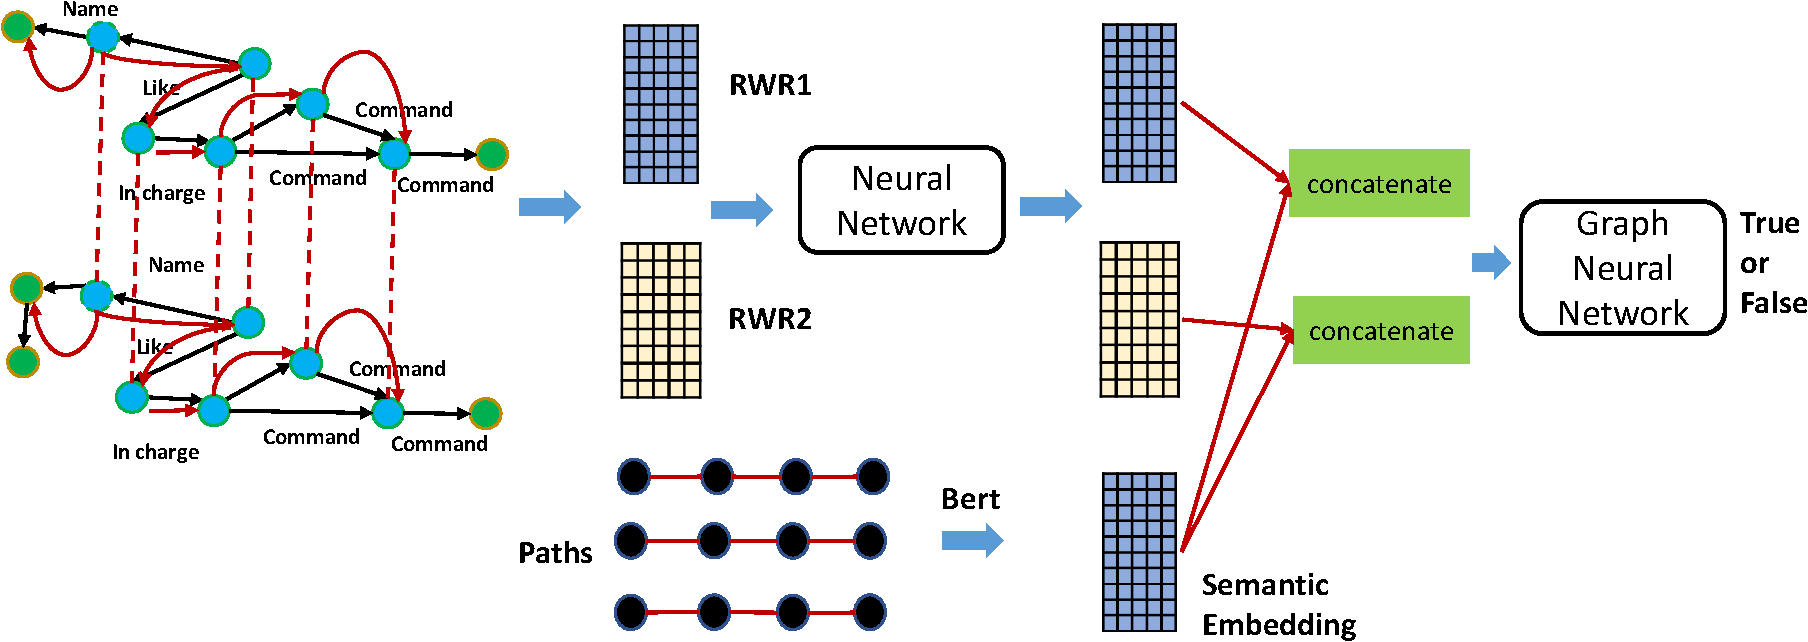
\includegraphics[width=0.9\textwidth]{submissions/logical-queries-uiuc/img/nn_pairwise_reasoning.pdf}
\caption{Neural network based pairwise comparative reasoning framework.
}
\label{nn_pairwise}
\end{figure*}

The pseudo code is given in Algorithm~\ref{pair_nn}. GNN means graph neural network which is defined as follows
\begin{equation}
    x^l_{N(u)} = \textrm{AGGREGATE}(\{\mathbf{X}^l(v,:), for v\in N(u)\})
\end{equation}
\begin{equation}
    \mathbf{X}^{l+1}(u,:) = \sigma(\textrm{CONCAT}(\mathbf{X}^l(u,:), x^l_{N(u)}))
\end{equation}
where AGGREGATE is the aggregation function, $\mathbf{X}$ is the input node embedding, $l$ is the graph neural network layer number, and $(u, v)$ are nodes in the input graph. The classifier in Algorithm~\ref{pair_nn} can be any machine learning model, e.g., SVM, logistic regression, decision tree and so on.

\begin{algorithm}[H] % algorithm begin
	\caption{Neural Network Based Pairwise Comparative Reasoning} % Algorithm title
	\label{pair_nn}
	\begin{algorithmic}[1]
		\STATE \textbf{Input:} Knowledge segment $KS_1$ and knowledge segment $KS_2$, pretrained embedding of all entities $\mathbf{E}$ in the knowledge graph.
		\STATE \textbf{Training:}
		\STATE Calculate random walks with restart matrices $\textrm{RWR}_1$  and $\textrm{RWR}_2$ for $KS_1$ and  $KS_2$, respectively.
		\STATE $E_{1}$ = NeuralNetwork($\textrm{RWR}_{1}$)
		\STATE  $E_{2}$ = NeuralNetwork($\textrm{RWR}_{2}$)
		\STATE Get all node embedding in $KS_1$: $N_{1}$ = $\mathbf{E}(KS_1)$
		\STATE Get all node embedding in $KS_2$: $N_{2}$ = $\mathbf{E}(KS_2)$
  	\STATE Concatenate embedding $C_1 = (E_{1} | N_{1})$
        \STATE Concatenate embedding $C_2 = (E_{2} | N_{2})$
        \STATE Predict result: Classifier(GNN($C_1$), GNN($C_2$))
	\end{algorithmic}
\end{algorithm}
\vspace{-1\baselineskip}

\subsection{Graph Kernel Based Pairwise Comparative Reasoning}

Different from neural network based pairwise comparative reasoning, graph kernel based pairwise comparative reasoning aims to utilize graph kernel to find a set of key elements (nodes or edges or node attributes) in these two knowledge segments and then make decision according to these elements and related information in the knowledge graph.
The idea is that if most of these key elements belong to the commonality of these two knowledge segments, it is highly likely that they refer to the same thing. Otherwise, these two clues refer to different things. Third, if they refer to the same thing, we further decide whether they conflict with each other. Here, the key idea is as follows. We build two new query triples $<{\tt o_1}$, {\tt isTypeOf}, ${\tt o_2}>$ and $<{\tt o_2}$, {\tt isTypeOf}, ${\tt o_1}>$. If one of them is true, the original two triples are consistent with each other. Otherwise, they are inconsistent.

In order to find the key elements, we propose to use the influence function w.r.t. the knowledge segment similarity \cite{qinghai}. The basic idea is that if we perturb a key element (e.g., change the attribute of a node or remove a node/edge), it would have a significant impact on the overall similarity between these two knowledge segments. Let $KS_1$ and $KS_2$ be the two knowledge segments.
We can treat the knowledge segment as an attributed graph, where different entities have different attributes.
We use random walk graph kernel with node attribute to measure the similarity between these two knowledge segments ~\cite{qinghai} ~\cite{sysvester}.

\vspace{-1\baselineskip}
\begin{eqnarray}\label{eq:rwgraphkernel}
\textrm{Sim}(KS_1, KS_2) = q'_{\times}(I - cN_{\times}A_{\times})^{-1}N_{\times}p_{\times}
\end{eqnarray}
where ${q'}_{\times}$ and $p_{\times}$ are the stopping probability distribution and the initial probability distribution of random walks on the product matrix, respectively. $N_{\times}$ is the combined node attribute matrix of the two knowledge segments $N_{\times} = \sum_{j=1}^d N_1^j \otimes N_2^j$ where $N_i^j$ ($i\in \{1,2 \}$) is the diagonal matrix of the $j^\textrm{th}$ column of attribute matrix $N_i$.
$A_{\times}$ is the Kronecker product of the adjacency matrices of knowledge segments $A_1$ and $A_2$. $0 < c < 1$ is a parameter.

We propose to use the influence function $\textrm{Sim}(KS_1 , KS_2)$ w.r.t. knowledge segment elements
 $\frac{\partial{Sim(KS_1, KS_2)}}{\partial {e}}$,
where $e$ represents an element of the knowledge segment $KS_1$ or $KS_2$.
The element with a high absolute influence function value is treated as a key element, and it can be a node, an edge, or a node attribute.
The influence function of different elements can be computed according to the following lemma.
Note that the influence function w.r.t. elements in $KS_2$ can be computed in a similar way.
\vspace{-0.3\baselineskip}
\begin{lemma}\label{lm:influence}\noindent (Knowledge Segment Similarity Influence Function ~\cite{qinghai}.)
Given $\textrm{Sim}(KS_1, KS_2)$
in Eq.~\eqref{eq:rwgraphkernel}.
Let $Q = (I - c N_{\times} A_{\times})^{-1}$ and $S^{j,i}$ is a single entry matrix defined in Table~\ref{notation}.
We have that
\item [] (i) The influence of an edge $A_1(i,j)$ in $KS_1$ can be calculated as
\begin{equation}
    I(A_1(i,j))= \frac{\partial \textrm{Sim}(KS_1, KS_2)}{\partial A_1(i,j)} =
c {q'}_{\times}QN_{\times}[(S^{i,j} + S^{j,i})\otimes A_2]QN_{\times}p_{\times}
\end{equation}


\item [] (ii) The influence of a node $i$ in $KS_1$ can be calculated as
\begin{equation}
    I(N_1(i)) = \frac{\partial \textrm{Sim}(KS_1, KS_2)}{\partial N_1(i)} =
c {q'}_{\times}QN_{\times}[\sum_{j|A_1(i,j)=1}(S^{i,j} + S^{j,i})\otimes A_2]QN_{\times}p_{\times}
\end{equation}


\item [] (iii) The influence of a node attribute $j$ of node $i$ in $KS_1$ can be calculated as
\begin{equation}
    I(N_1^j(i, i)) = \frac{\partial \textrm{Sim}(KS_1, KS_2)}{\partial N_1^j(i, i)} =
q'_{\times}Q[S^{i,i}\otimes N_2^j](I + c A_{\times}QN_{\times})p_{\times}
\end{equation}


%\hh{(1) check if the equation are correct. (2) and if we need to explain additional notations.}
\end{lemma}
\vspace{-0.3\baselineskip}



For a given knowledge segment, we flag the top 50\% of the elements (e.g., node attribute, node and edge) with the highest absolute influence function values as key elements.
We would like to check whether these key elements belong to the commonality of these two knowledge segments. If most of them (e.g., 60\% or more) belong to the commonality of these two knowledge segments, we say the two query clues describe the same thing. Otherwise, they refer to different things and thus we do not need to check the inconsistency between them.

If we determine that the query clues refer to the same thing, the next step is to decide whether they are inconsistent with each other. That is, given query clues $<{\tt s_1}$, ${\tt p_1}$, ${\tt o_1}>$ and $<{\tt s_1}$, ${\tt p_2}$, ${\tt o_2}>$, we need to decide whether ${\tt o_1}$ belongs to ${\tt o_2}$ or ${\tt o_2}$ belongs to ${\tt o_1}$.
To this end, we build two new queries $<{\tt o_1}$, {\tt isTypeOf}, ${\tt o_2}>$ and $<{\tt o_2}$, {\tt isTypeOf}, ${\tt o_1}>$. Then, we extract the knowledge segments for these two queries, and check whether these two segments are true. If one of them is true, we say the original clues are consistent with each other, otherwise they are inconsistent.
After we extract the knowledge segments for $<{\tt o_1}$, {\tt isTypeOf}, ${\tt o_2}>$ and $<{\tt o_2}$, {\tt isTypeOf}, ${\tt o_1}>$, we treat each knowledge segment as a directed graph, and calculate how much information can be transferred from the subject to the object. We define the transferred information amount %\hh{let us use 'transferred information amount' consistently}
as:
\begin{equation}\label{eq:transinfo}
    \textrm{infTrans}({\tt o_1}, {\tt o_2}) = \max_{1 \leq j \leq k} \textrm{pathValue}(j)
\end{equation} where $\textrm{pathValue}(j)$ is defined as the multiplication of the weights in the path. For an edge, its weight is the predicate-predicate similarity $\textrm{Sim}({\tt isTypeOf}, e_i)$. If $\max\{\textrm{infTrans}({\tt o_1}, {\tt o_2}),  \textrm{infTrans}({\tt o_2}, {\tt o_1})\}$ is larger than a threshold $T$, then we say ${\tt o_1}$ belongs to ${\tt o_2}$ or ${\tt o_2}$ belongs to ${\tt o_1}$. We set $T = 0.700$ in our experiment.

\hide{
\begin{figure}
	\centering
	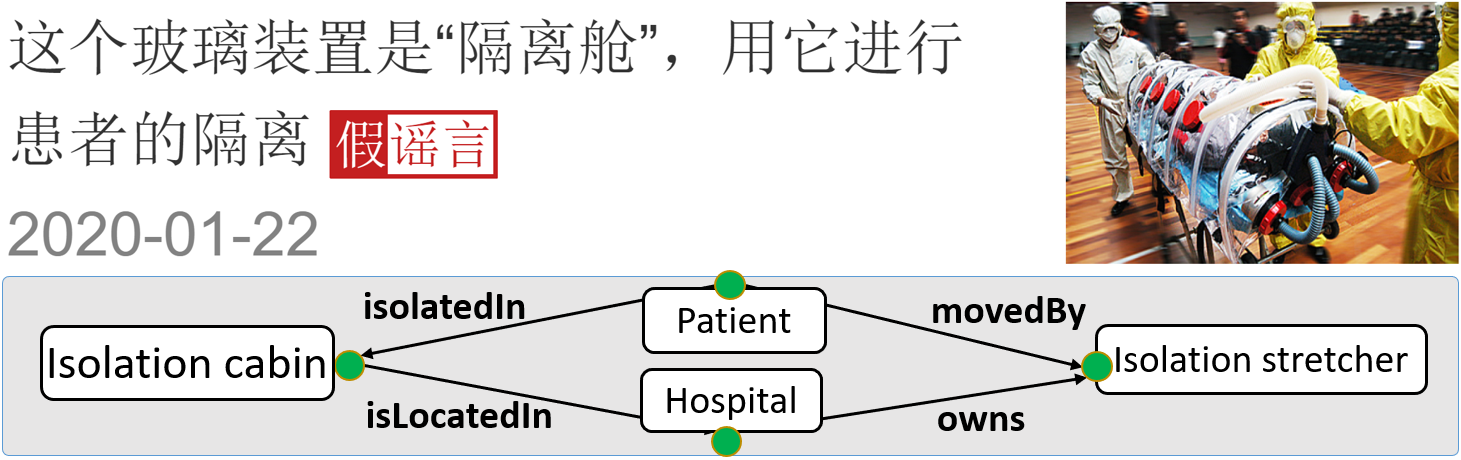
\includegraphics[width=0.43\textwidth]{img/qq_example.png}
	\vspace{-1\baselineskip}
	\caption{A fake news example from Wuhan coronavirus crisis. The text in the news says ``{\em This glass device is `Isolation Cabin', which is used to  isolate patients.}".}
	\label{qq_example}
	\vspace{-1\baselineskip}
\end{figure}


Let us take an example from Wuhan coronavirus crisis which is shown in Figure ~\ref{qq_example}.
The query we get from text is $<${\tt Patient}, {\tt isolatedIn}, {\tt Isolation Cabin}$>$,
and the query we get from image is $<${\tt Patient}, {\tt isolatedIn}, {\tt Isolation stretcher}$>$.
To detect the inconsistency of this pair of clues, we only need to check whether $<${\tt Isolation Cabin}, {\tt isTypeOf}, {\tt Isolation stretcher}$>$ or $<${\tt Isolation stretcher}, {\tt isTypeOf}, {\tt Isolation Cabin}$>$.
If we have $\textrm{infTrans}({\tt Isolation~Cabin}, {\tt Isolation~stretcher}) < 0.700$ based on the knowledge segment extracted from the knowledge graph, we conclude that Isolation Cabin is not Isolation stretcher. Therefore, there exists inconsistency in this news.% about Wuhan coronavirus crisis.
}

%%%%%%%%%%%%%%%%%%%%%%%%%%%%%%%%%%%%%%%%%%%%%%%%%%%%%%%%%%%%%%%%%%%%%%%%%%%%%%%%%%%%%%%%%%%%%%%%%%%%%%%%%%%%%%


\subsection{Graph Kernel Based Collective Comparative Reasoning}

%In last section, we introduce the pairwise comparative reasoning. In this section, we introduce collective comparative reasoning.
Different from pairwise comparative reasoning, collective comparative reasoning aims to find the commonality and/or inconsistency inside a query graph which consists of a set of inter-connected edges/triples.
To check the inconsistency, one naive method is using the pairwise comparative reasoning method to check the inconsistency for each pair of edges in the query graph. However, this method is neither computationally efficient nor sufficient. For the former, if two clues (e.g., two claims from a news article) are weakly or not related with each other on the query graph, we might not need to check the inconsistency between them at all. For the latter, in some subtle situations, the semantic inconsistencies could {\em only} be identified when we collectively reason over multiple (more than two) knowledge segments. For example, given the following three claims, including
(1) {\em Obama is refused by Air Force One};
(2) {\em Obama is the president of the US};
(3) {\em The president of US is in front of a helicopter}.
Only if we reason these three claims collectively, can we identify the semantic inconsistency among them.
%In other cases, the additional claim (e.g., <Marine One, max distance, 600M>) and its corresponding knowledge segment might provide extra corroborations for pairwise semantic inconsistency reasoning (e.g., <Obama, field, 6,000M> and <Obama, in front of, Marine One>).

%The idea behind collective comparative reasoning is that if the query graph is consistent, the semantic matching subgraph should contain no inconsistency.
Based on the above observation, we propose the following method to detect the collective inconsistency.%\bx{'First' goes to a new line?}

\textbf{First}, we find a set of key elements inside the semantic matching subgraph.
Different from pair-wise comparative reasoning, the importance/influence of an element for collective comparative reasoning is calculated by the entire semantic matching subgraph.
More specifically,
we first transform the query graph and its semantic matching subgraph (i.e., subgraph-specific knowledge segment) into two line graphs, which are defined as follows.
\vspace{-0.5\baselineskip}
\begin{definition} {\bf Line Graph~\cite{Shiralkar2017}}.
For an arbitrary graph $G=(V, E)$, the line graph $L(G) = (V', E')$ of  $G$ has the following properties:
(1) the node set of $L(G)$ is the edge set of $G$ ($V' = E$);
(2) two nodes $V'_i$, $V'_j$ in $L(G)$ are adjacent if and only if the corresponding edges $e_i$, $e_j$ of $G$ are incident on the same node in $G$.
\end{definition}
\vspace{-0.5\baselineskip}
Figure ~\ref{collective-compare-workflow} gives an example of the line graph.
For the line graph $L(Q)$, the edge weight is the predicate-predicate similarity of the two nodes it connects.
For the line graph $L(KS)$, the edge weight is the knowledge segment similarity by Eq.~\eqref{eq:rwgraphkernel} of the two nodes it connects.
The rationality of building these two line graphs is that if the semantic matching subgraph is a good representation of the original query graph, the edge-edge similarity in $L(Q)$ would be similar to the knowledge segment similarity in $L(KS)$.

\begin{figure}
	\centering
	\vspace{-1\baselineskip}
	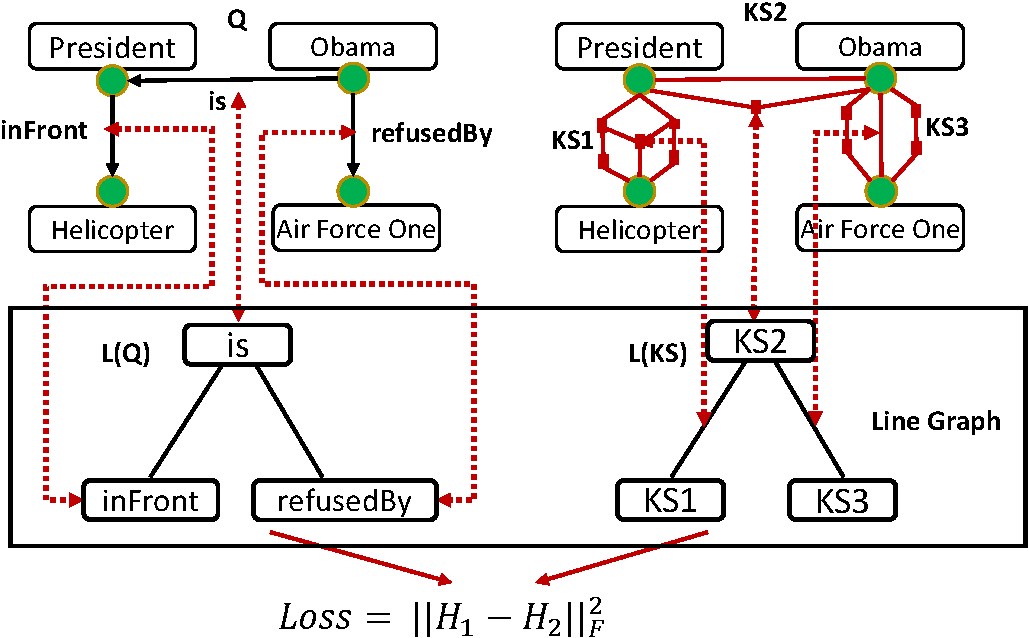
\includegraphics[width=0.5\textwidth]{submissions/logical-queries-uiuc/img/line-loss.pdf}
	\caption{Collective comparative reasoning workflow.}
	\label{collective-compare-workflow}
	\vspace{-1\baselineskip}
\end{figure}

To measure the importance of an element, we propose to use the influence function w.r.t. the distance between $L(Q)$ and $L(KS)$. We assume that a key element, if perturbed, would have a great effect on the distance
$\textrm{Loss} = || H_1 - H_2 ||_F^2$
%\hh{W1 and W2 have already been used in predicate-predicate similarity}
, where $H_1$ is the weighted adjacency matrix of $L(Q)$, and $H_2$ is the weighted adjacency matrix of $L(KS)$. We use the influence function $\frac{\partial \textrm{Loss}(H_1, H_2)}{\partial e}$, where $e$ represents an element of the knowledge segment graph and it could be a node, an edge, or a node attribute. Lemma~\ref{lm:collectiveinfluence} provides the details on how to compute such influence functions.

%If there are inconsistency in the query graph, after we correct such wrong node/edge attributes, it would significantly reduce the loss function. To this end,


\begin{lemma}\label{lm:collectiveinfluence}
Given the loss function $Loss = || H_1 - H_2 ||_F^2$. Let $n$, $k$ denote two different nodes in $L(Q)$,
and $KS_n$, $KS_k$ denote their corresponding knowledge segments.
Let $h_{e_{k,n}}$ denote the weight of edge between node $k$ and $n$,  and $h_{c_{k,n}}$ denote the weight of edge between $KS_k$ and $KS_n$. We have

\item [] (i) The influence of an edge $A_n(i,j)$ in knowledge segment $KS_n$ can be calculated as

$I(A_n(i,j)) = \sum_{k \in N(n)} -2(h_{e_{k,n}} - h_{c_{k,n}})\frac{\partial sim(KS_n, KS_k)}{\partial A_n(i,j)}$.

\item [] (ii) The influence of a node $i$ in knowledge segment $KS_n$ can be calculated as

$I(N_n(i)) = \sum_{k \in N(n)} -2(h_{e_{k,n}} - h_{c_{k,n}})\frac{\partial sim(KS_n, KS_k)}{\partial N_n(i)}$.

\item [] (iii) The influence of a node attribute $j$ in knowledge segment $KS_n$ can be calculated as

$I(N_n^j(i,i)) = \sum_{k \in N(n)} -2(h_{e_{k,n}} - h_{c_{k,n}})\frac{\partial sim(KS_n, KS_k)}{\partial N_n^j(i,i)}$.

\end{lemma}

\begin{proof}
We rewrite the loss function as
\setlength{\abovedisplayskip}{1pt}
\setlength{\belowdisplayskip}{1pt}
\begin{small}
\[
Loss = || H_1 - H_2 ||_F^2 = \sum_{i,j} (h_{e_{i,j}} - h_{c_{i,j}})^2
\vspace{-0.6\baselineskip}
\]
Take the derivative, together with Lemma 1, we have
\begin{equation}
\begin{aligned}
I(A_n(i,j)) &= \sum_{k \in N(n)} -2(h_{e_{k,n}} - h_{c_{k,n}})\frac{\partial sim(KS_n, KS_k)}{\partial A_n(i,j)} \\
\vspace{-0.6\baselineskip}
(N_n(i)) &= \sum_{k \in N(n)} -2(h_{e_{k,n}} - h_{c_{k,n}})\frac{\partial sim(KS_n, KS_k)}{\partial N_n(i)}  \\
I(N_n^l(i,i)) &= \sum_{k \in N(n)} -2(h_{e_{k,n}} - h_{c_{k,n}})\frac{\partial sim(KS_n, KS_k)}{\partial N_n^l(i,i)}
\end{aligned}
\end{equation}
\end{small}
which completes the proof.
\end{proof}


\textbf{Second}, after we find all the key elements, we check the consistency of the semantic matching subgraph according to these key elements. The steps are as follows.
For each pair of knowledge segments of the  semantic matching subgraph, if their key elements overlapping rate is greater than a threshold (60\%), we check the consistency of this pair. Suppose the corresponding triples are $<{\tt s_1}$, ${\tt p_1}$, ${\tt o_1}>$ and $<{\tt s_2}$, ${\tt p_2}$, ${\tt o_2}>$, respectively. We check if $<{\tt s_1}$, {\tt isTypeOf}, ${\tt s_2}>$ or $<{\tt s_2}$, {\tt isTypeOf}, ${\tt s_1}>$ is true. If both of them are false, we skip this pair of clues because it does not belong to C3 or C4. Otherwise, we check if $<{\tt o_1}$, {\tt isTypeOf}, ${\tt o_2}>$ or $<{\tt o_2}$, {\tt isTypeOf}, ${\tt o_1}>$ is true. If both of them are false, we say this query graph has collective inconsistency. When checking the truthfulness of triples (e.g., $<{\tt s_1}$, {\tt isTypeOf}, ${\tt s_2}>$,
$<{\tt s_2}$, {\tt isTypeOf}, ${\tt s_1}>$,
$<{\tt o_1}$, {\tt isTypeOf}, ${\tt o_2}>$ and $<{\tt o_2}$, {\tt isTypeOf}, ${\tt o_1}>$),
we use the same method (i.e., transferred information amount in Eq.~
\eqref{eq:transinfo}) as in pairwise comparative reasoning. 